We now discuss our primary contribution; a parallelized version of the
model described in \cite{goldwater2011}. Such a model is attractive
because it has the potential to allow unsupervised morphological
induction procedures to scale large datasets. In Section~\ref{sec:evaluation},
we will show that our new model is just as
accurate as the baseline model. This confirms that the auxiliary
variables used to introduce the independencies exploited for
parallelization do not affect the model's correctness. We believe this
result is non-trivial because the parallel DPMM described by
\cite{williamson2013} is designed with Gaussian mixture models in mind
where the base distribution $H$ is of little interest. In our model,
however, the base distribution encodes the knowledge that we are most
interested in discovering within a language (the distribution over
prefixes and suffixes). We also show that our parallelized model is
able to compute a full iteration of the Gibbs sampler much more
quickly than a comparable serialized model.

The variables used in our parallelized model are a superset of those
used in the baseline model. We review them below

\begin{itemize}

\item $\alpha$ together with the fixed number of compute nodes (or
  processors) $P$ parameterize two distributions in our model. First,
  $\alpha/P$ parameterizes the symmetric Dirichlet prior over the
  processor multinomial $\phi$. Second, $\alpha/P$ also acts as the
  concentration parameter of the DP over $G_{1:P}$.

\item $\alpha_p$ and $\alpha_s$ are the concentration parameters of
  the symmetric Dirichlet priors over $\theta_p$ and $\theta_s$
  respectively.

\item The base distribution $H$ is a distribution over prefix-suffix
  tuples $(p, s)$ and is defined to be $H(p, s) = p(p | \theta_p) p(s
  | \theta_s)$.

\item The $P$ random measures $G_{1:P}$ are independent draws from the
  Dirichlet process parameterized with concentration parameter
  $\alpha/P$ and base distribution $H$.

\item $\phi$ is a multinomial distribution over processors. This is
  used to choose a processor assignment for a particular word in the
  generative process.

\item $\pi_i \in \{1, \ldots, P\}$ is the processor assignment for
  each word $w_i$. Conditioned on this variable, the seating
  assignments for words on processor $\pi$ can be resampled
  independently.

\item $(p_i, s_i)$ are the set of parameters sampled from the random
  measure $G_{\pi_i}$. These are concatenated to form a ``draw'' from
  the distribution $f(p_i, s_i)$, which is determinstically the word
  formed by the concatenation of $p_i$ and $s_i$ (i.e. $w_i = p_i +
  s_i$).

\end{itemize}

The generative story for this model can be seen below, and a
visualization can be seen in Figure \ref{fig:v3}.

\begin{align*}
  \theta_p & \sim \Dir(\alpha_p) \\
  \theta_s & \sim \Dir(\alpha_s) \\
  H(p, s) & = p(p \mid \theta_p) p(s \mid \theta_s) \\
  \phi & \sim \Dir\left(\frac{\alpha}{P}\right) \\
  \forall j \in \{1 \dots P\} \\
  G_j & \sim \DP\left(\frac{\alpha}{P}, H\right)\\
  \forall i \in \{1 \dots N\} \\
  \pi_i & \sim \phi \\
  (p_i, s_i) & \sim G_{\pi_i} \\
  w_i & = p_i+s_i
\end{align*}

\begin{figure}[h]
  \centering
  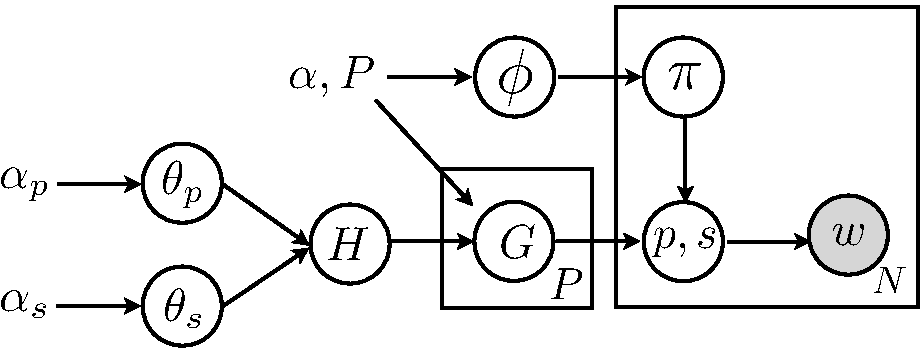
\includegraphics[width=0.6\textwidth]{fig/v3}
  \caption{Parallelized model}
  \label{fig:v3}
\end{figure}

It is important to note a key difference between the model presented
in \cite{williamson2013} and the model presented here. The
parallelized DPMM can take advantage of the fact that the base
distribution is relatively simple in order to simplify the amount of
global synchronization that must be done. Specifically,
\cite{williamson2013} test their parallelized algorithm on synthetic
data generated from a mixture of univariate one dimensional Gaussians
with means sampled from a uniform distribution $Unif(0, 10)$ and a
fixed variance (set to $0.1$). Inference in this model moves between
local resampling in each of the $P$ CRPs and global resampling of the
processor indicators $\pi_{1:n}$. Since the variables of interest are
the cluster indicators $Z^n$ and the means of each cluster, there is
no need for the local CRPs to communicate any information to the
master node.

In our model, however, the variables of interest are $\theta_p$ and
$\theta_s$; the distributions over prefixes and suffixes that allow us
to decode any given token once the model has been learned. We believe
that this is an important difference, as it required a significant
amount of additional effort in the implementation to coordinate
intricate global synchronization among local CRPs and the master node
(the processor that keeps track of the base and directs the local
CRPs---this is discussed further in the section on inference). We
discuss our implementation further in the following section.

\subsection{Inference in the Parallel Model}

Given a particular value of the parameter $P$, we involve $P + 1$
processors or compute nodes in the computation. One node, which we
call the \textit{master}, coordinates inference among the other nodes,
which we call the \textit{slaves}. Communication is bidirectional, but
proceeds in a query-respond fashion, where the master node asks the
slaves to compute certain values or take certain inferential steps,
and slaves respond with values required by the master node to take
global inference steps. Pseudo code for the algorithm can be found in
Figure~\ref{fig:inference}.

At a high level, parallelized inference in our model proceeds in two
stages that alternate until convergence. The local stage is composed
of $P$ parallel Chinese restaurant processes being run on the $P$
slave nodes. During initialization, word $w_i$ is randomly assigned to
a processor with probability $1/P$ (assignments are resampled---we
describe the procedure later). The Dirichlet process from which we are
implicitly sampling is $DP(\alpha/P, H)$, where the random measure
$G_j$ for processor $j$ has been marginalized out. In terms of the
restaurant metaphor, the customers are all words $w_i : {\pi_i =
  j}$. For each local iteration, a slave first resamples the seating
arrangements of each customer, and then resamples the dishes assigned
to each table given the current, fixed base distribution $H$. It is,
however, important to note that an implementation must keep explicit
track of each table, its dish, and the number of customers at the
table (or each slave node must be able to compute this from the
information it does store). The information about each table is
necessary for the global inference steps and will be communicated to
the master node. This is one of the key differences between what is
necessary for our model and what is necessary for the Gaussian DPMM
discussed in \cite{williamson2013}.

Globally, after each of the slaves has completed a single iteration of
the CRP, the master node receives a message from each slave containing
the number of times each prefix and each suffix occurs on a table in
the slave's local CRP. These counts are recorded in the base
distribution $H$, and a new $\theta_p$ and $\theta_s$ are drawn from
the following distributions where $\#p_i, \#s_j$ is the number of times
the $i$th prefix and $j$th suffix respectively occurs on any table in
any of the local restaurants, and where $|p|, |s|$ are the total
number of prefixes and suffixes in the model.

\begin{align}
  \theta_p^{t+1} & \sim p(\theta_p | \text{table counts}, \alpha_p) = \Dir(\#p_1 + \alpha, \ldots, \#p_{|p|} + \alpha) \\
  \theta_s^{t+1} & \sim p(\theta_s | \text{table counts}, \alpha_s) = \Dir(\#s_1 + \alpha, \ldots, \#p_{|s|} + \alpha)
\end{align}

After a new $\theta_p^{t+1}, \theta_s^{t+1}$ pair has been sampled,
this defines a new base distribution $H^{t+1}$. This new base
distribution is fixed, and passed back to the slaves to be used in the
next iteration of inference when resampling dishes for each table.

In our implementation most of the variables introduced for
parallelization are marginalized. The multinomial $\phi$ is
marginalized out, and so are each of the random measures $G_j : j \in
\{1, \ldots, P\}$. The processor indicators $\pi_i$, however, cannot
be marginalized out, and so we must resample them to ensure that our
model mixes correctly. Following \cite{williamson2013}, we resample
processor indicators using a Metropolis Hastings step by resampling
the processor indicators for entire tables. To coordinate this
transition, the master node asks each slave node for a list of
2-tuples where each tuple corresponds to a single table in the slave's
restaurant. The first element of the tuple is a prefix-suffix pair (a
dish) and the second element is the number of customers sitting at
that table. With this information collected from each slave, the
master then resamples processor indicators \textit{for each table}
(i.e.~we resample a new $\pi$ simultaneously for each customer at the
table) by drawing from a uniform distribution over the processors. We
accept the transition with probability $\min(1, r)$ where r is defined
as

\begin{align}
  r = \prod_{j = 1}^P \prod_{i=1}^{\max(N_j, N_j^*)} \frac{a_{ij}!}{a_{ij}^*!}
\end{align}

where $N_j$ is the number of words on processor $j$ in the old
configuration, $N_j^*$ is the number of words on processor $j$ in the
new configuration, and $a_{ij}, a_{ij}^*$ is the number of tables with
$i$ customers on processor $j$ for the old and new configuration
respectively. This quantity is simply the likelihood ratio of the new
configuration to the old configuration. We omit its derivation, but it
can be found in the supplementary material of
\cite{williamson2013}. If new processor indicators have been assigned,
a list of 2-tuples is sent back to each of the slaves (the slave's new
tables with dishes and counts), and the slave can then rebuild its
internal data structures to continue inference.

\begin{figure}[h]
  \centering
  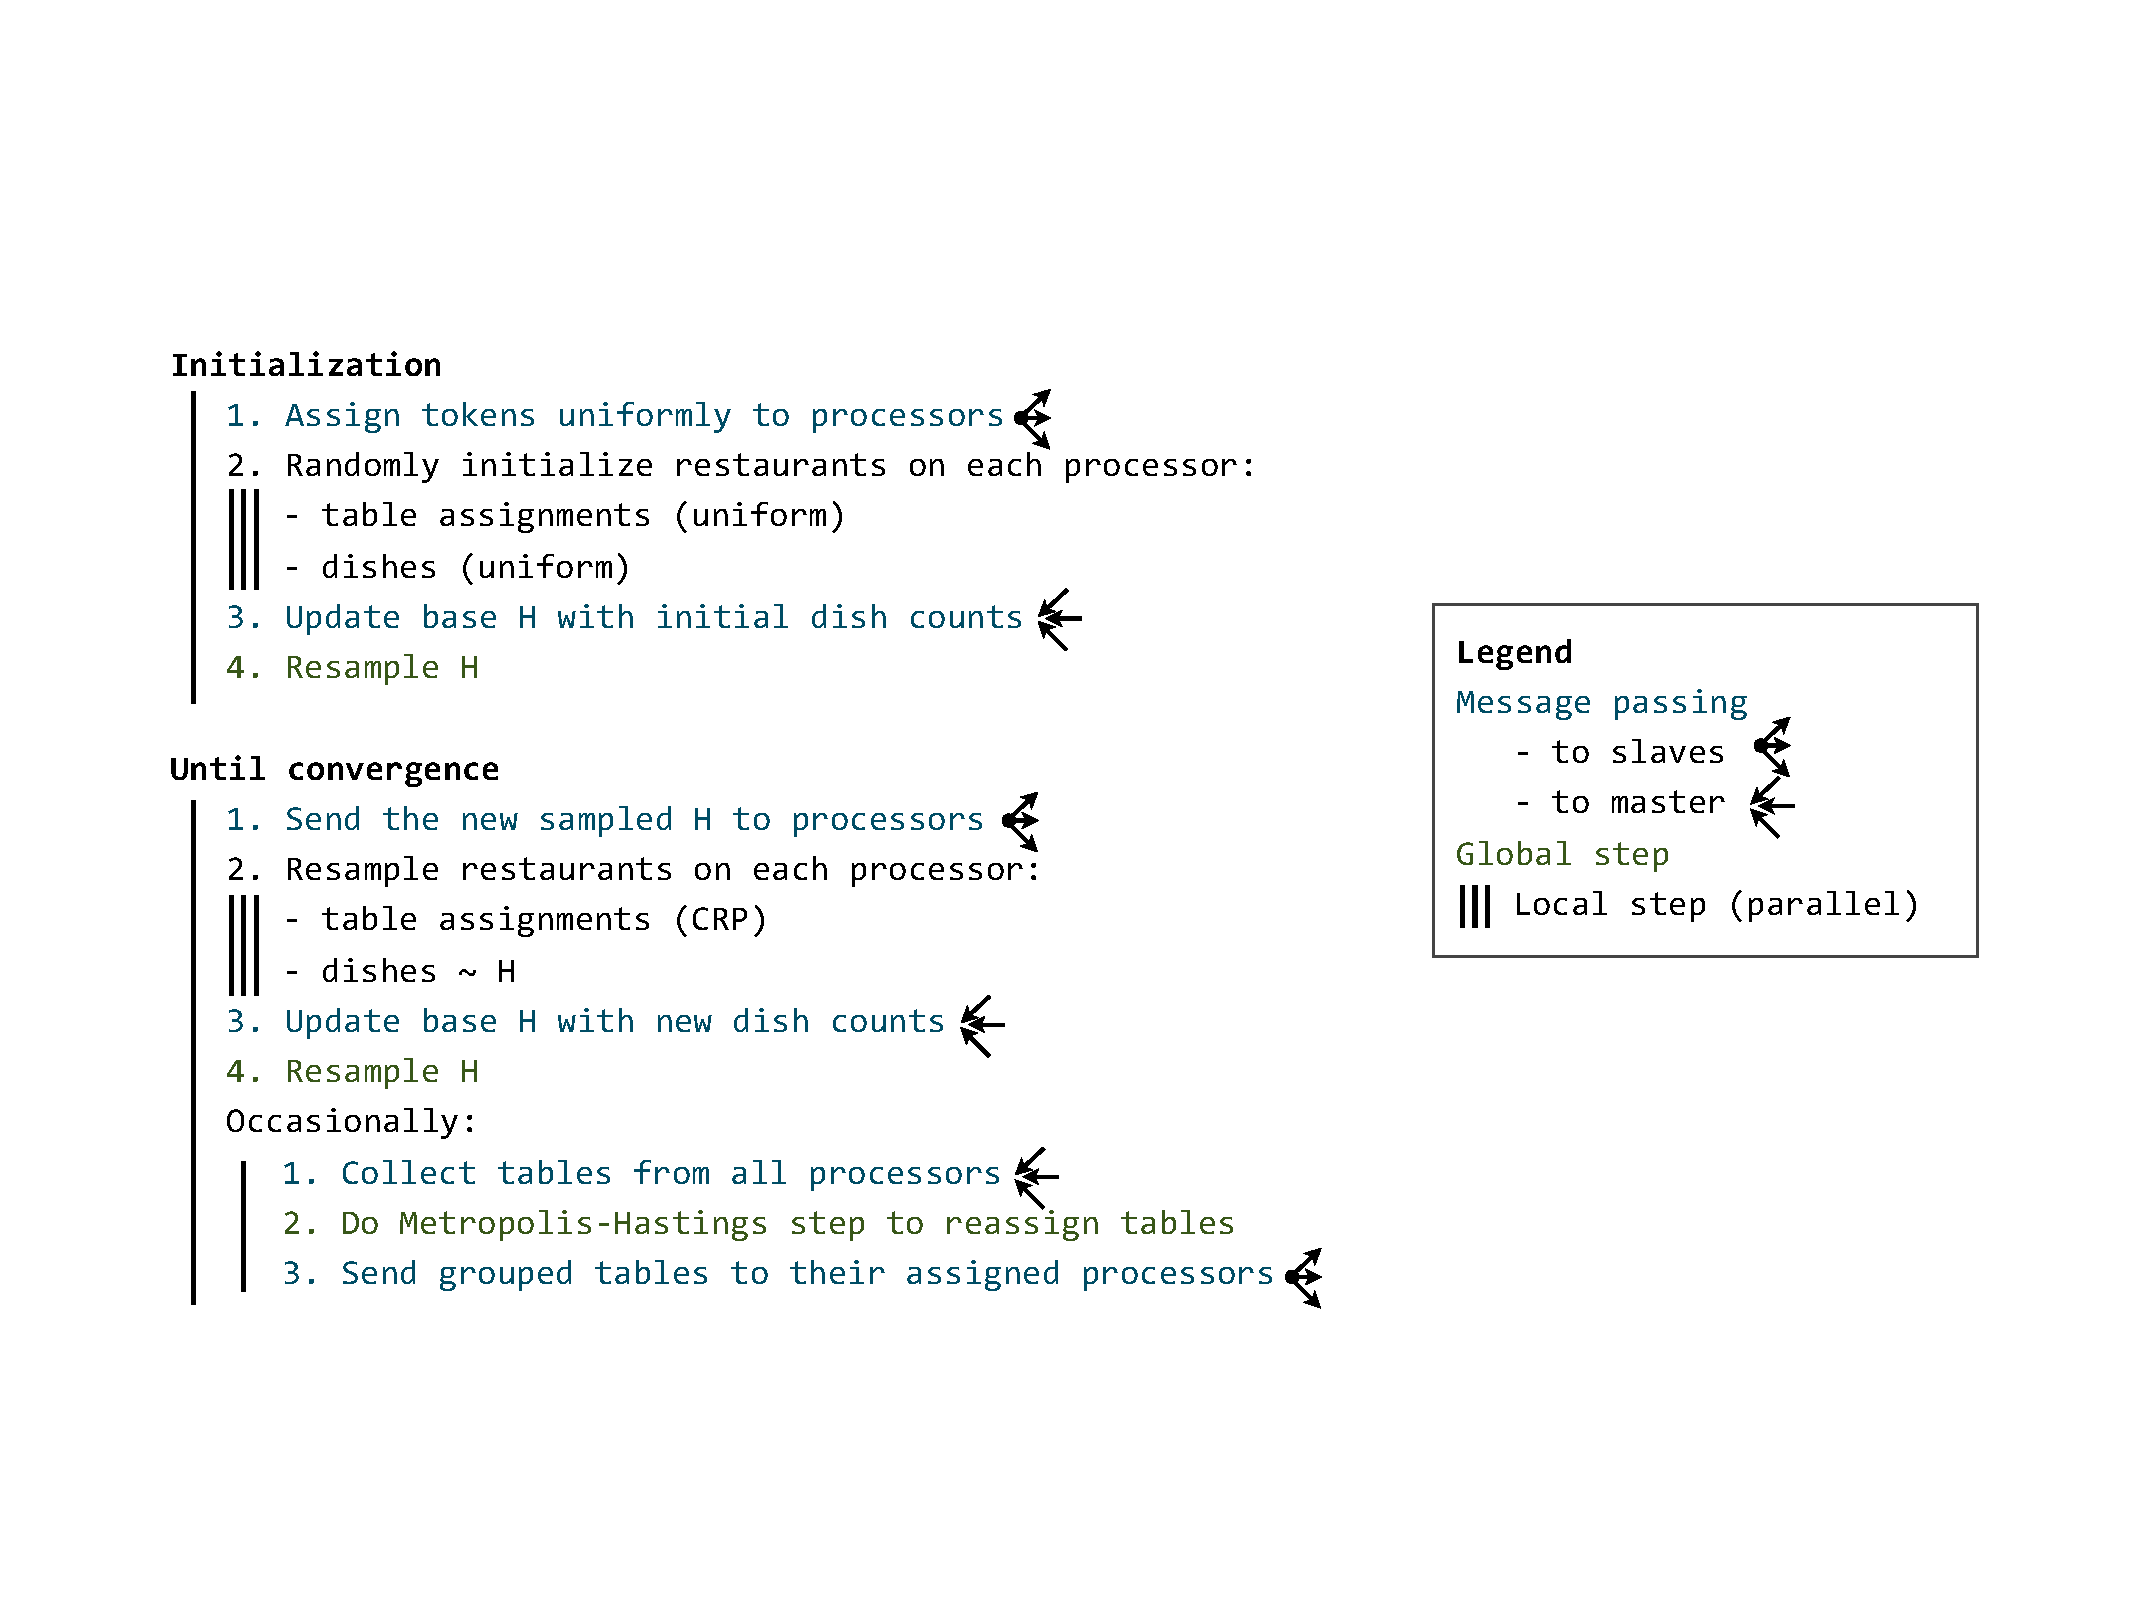
\includegraphics[width=1.05\textwidth]{fig/parallel_code_schema}
  \caption{Pseudo code for inference in the parallel model}
  \label{fig:inference}
\end{figure}
